\section{Разработка технического задания на модернизацию системы видеонаблюдения}

\subsection{Выбор топологии}

При топологии «звезда» каждая камера подключается по 1 кабелю к общему сетевому оборудованию (коммутатор, маршрутизатор).
Среди основных достоинств такой топологии расширяемость и управляемость. подводится к ее низкая стоимость, легкость подключения, отличная модернизация СКС.
Недостатки топологии «звезда», предполагает достаточно высокую стоимость внедрения и большое количество кабеля, а при отказе сетевого оборудования от сети 
отключаются все подцепленные к нему устройства системы видеонаблюдения.

\subsection{Выбор и описание параметров видеооборудования}

Видеооборудование было выбрано от компании TRASSiR\@.
Компания TRASSiR является одним из ведущих разработчиков решений в области информационных технологий и автоматизации процессов мониторинга и управления.
Основанная в 2007 году, TRASSiR сосредоточена на разработке и внедрении программных продуктов, предназначенных для повышения эффективности работы организаций различных отраслей.

Была выбрана модель видеокамеры TR-D2D2 v3 2.7-13.5, т.к. она подходит по основным необходимым параметрам.
Внешний вид видеокамеры показан на рисунке~\ref{fig::tr-d2d2}:

\begin{figure}[h]
    \begin{center}
        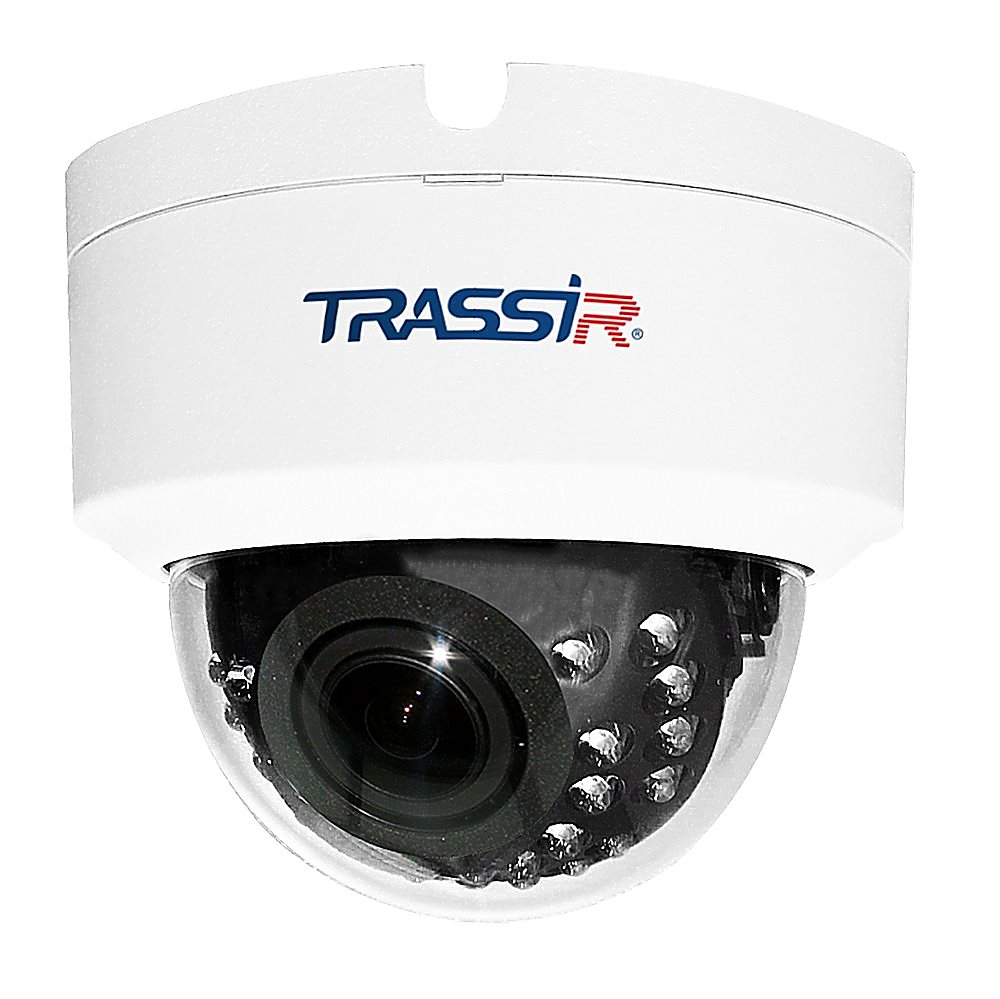
\includegraphics[width=50mm]{images/TR-D2D2}
    \end{center}
    \captionsetup{justification=centering}
    \caption{Внешний вид видеокамеры TR-D2D2}
    \label{fig::tr-d2d2}
\end{figure}

Технические характеристики указаны в таблице~\ref{tab::tr-d2d2-parameters}:
\begin{longtable}{|p{5cm}|p{12cm}|}
    \caption{Технические характеристики видеокамеры TR-D2D2 v3 2.7-13.5}
    \label{tab::tr-d2d2-parameters} \\

    \hline
    Параметр &
    Данные \\
    \hline
    Класс защиты &
    Нет \\
    \hline
    Детектор движения &
    Да \\
    \hline
    Кнопка сброса &
    Нет \\
    \hline
    Локальное хранилище &
    Нет \\
    \hline
    Улучшение изображения &
    3D DNR | BLC | Defog \\
    \hline
    Число пикселей &
    2 Мп \\
    \hline
    Тип объектива &
    С переменным фокусным расстоянием \\
    \hline
    Фокусное расстояние, мм &
    2.7 - 13.5 \\
    \hline
    Угол обзора H° &
    100 - 28 \\
    \hline
    Угол обзора V° &
    55 - 16 \\
    \hline
    Угол обзора D° &
    Нет \\
    \hline
    Сетевой интерфейс &
    RJ-45 \\
    \hline
    Видеосжатие &
    H.264, H.265, H.265+ \\
    \hline
    Поддержка RTSP &
    Да \\
    \hline
    Матрица &
    1/2.9'' CMOS \\
    \hline
    Максимальное разрешение &
    1920x1080 \\
    \hline
    Светочувствительность, Lux &
    0,003 \\
    \hline
    Питание &
    DC 12 В, PoE \\
    \hline
\end{longtable}

\newpage

В качестве коммутатора был выбран коммутатор от компании TRASSiR TR-NS1126-225-24PoE.
Внешний вид видеокамеры показан на рисунке~\ref{fig::TR-NS1126-225-24PoE}:

\begin{figure}[h]
    \begin{center}
        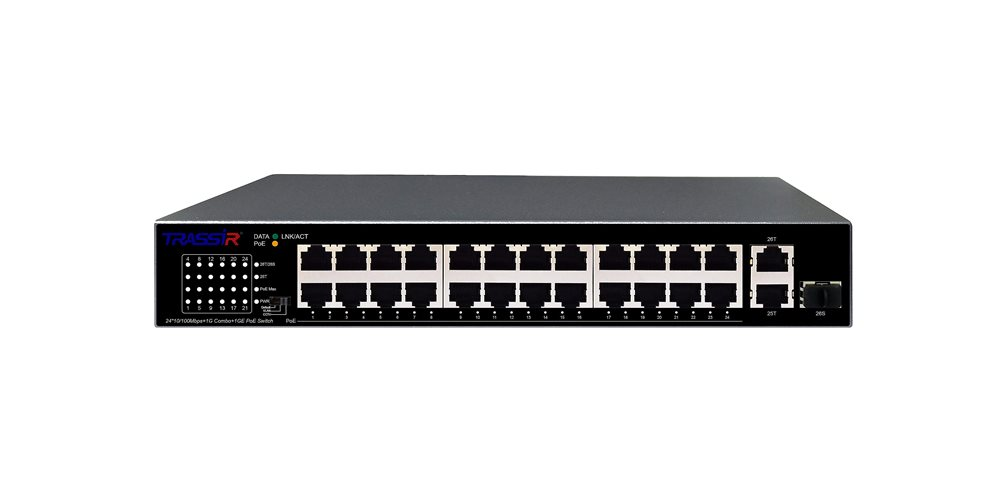
\includegraphics[width=120mm]{images/TR-NS1126-225-24PoE}
    \end{center}
    \captionsetup{justification=centering}
    \caption{Внешний вид коммутатора TR-NS1126-225-24PoE}
    \label{fig::TR-NS1126-225-24PoE}
\end{figure}

Технические характеристики указаны в таблице~\ref{tab::TR-NS1126-225-24PoE-parameters}:
\begin{longtable}{|p{5cm}|p{12cm}|}
    \caption{Технические характеристики коммутатора ЕR-NS1126-225-24PoE}
    \label{tab::TR-NS1126-225-24PoE-parameters} \\

    \hline
    Параметр &
    Данные \\
    \hline
    Управление &
    Нет \\
    \hline
    Таблицы MAC-адресов, К &
    16 \\
    \hline
    Скорость обслуживания пакетов, Mpps &
    6,5 \\
    \hline
    Способ монтажа &
    В стойку / на плоскую поверхность \\
    \hline
    Питание &
    DC 55 В \\
    \hline
    Количество портов PoE &
    24 \\
    \hline
    Количество SFP портов &
    1 \\
    \hline
\end{longtable}

\newpage
В качестве видеорегистратора был выбран коммутатор от компании TRASSiR DuoStation AF Pro 16-RE
Внешний вид видеорегистратора показан на рисунке~\ref{fig::recorder}:

\begin{figure}[h]
    \begin{center}
        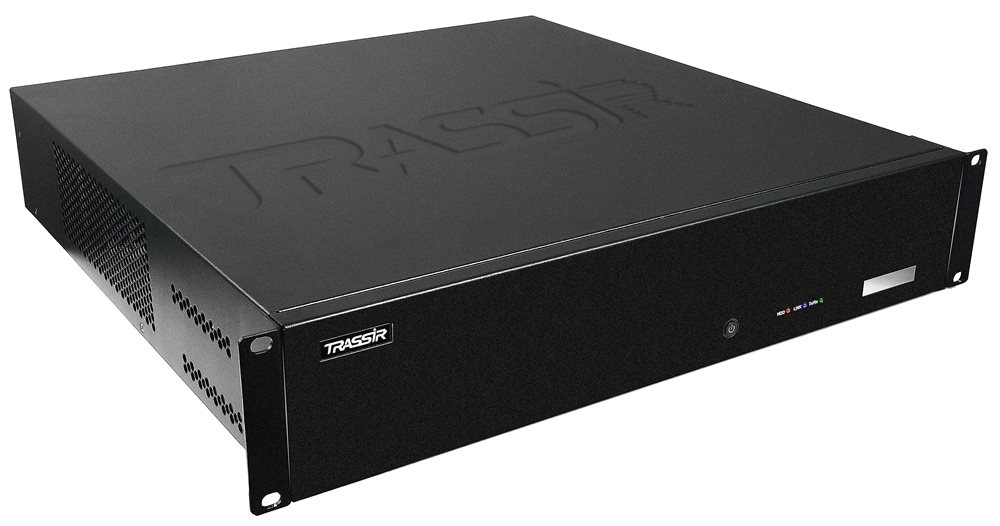
\includegraphics[width=80mm]{images/DuoStation AF Pro 16-RE}
    \end{center}
    \captionsetup{justification=centering}
    \caption{Внешний вид видеорегистратора DuoStation AF Pro 16-RE}
    \label{fig::recorder}
\end{figure}

Технические характеристики указаны в таблице~\ref{tab::recorder-parameters}:
\begin{longtable}{|p{5cm}|p{12cm}|}
    \caption{Технические характеристики видеорегистратора DuoStation AF Pro 16-RE}
    \label{tab::recorder-parameters} \\

    \hline
    Параметр &
    Данные \\
    \hline
    Формат видеосжатия &
    H.265+ | H.265 | H.264 | MJPEG | MPEG4 \\
    \hline
    Объем HDD, TB &
    16 \\
    \hline
    Сетевые протоколы &
    TCP/IP, IPv4/v6, UDP, DHCP, CloudConnect, DNS, NTP, SADP, SMTP, iSCSI, UPnP, HTTP/HTTPS, RTSP, ONVIF \\
    \hline
    Сетевые интерфейсы &
    2 RJ-45 10M/100M/1000M Ethernet \\
    \hline
    Кол-во IP каналов &
    16 \\
    \hline
    Основной поток записи, Мп &
    8 \\
    \hline
    Количество SFP портов &
    1 \\
    \hline
\end{longtable}

\subsection{Разработка плана размещения видеокамер}

Размещение видеокамер на объекте было рассчитано с учетом технических характеристик выбранных камер. 
На помещения с площадью меньше 22 м2 выделено по 1 видеокамере направленной из 1 угла комнаты в сторону входной двери, для её контроля. 
На помещения превышающие площадь 22 м2 используется по 2 видеокамеры направленных друг на друга с целью предотвращения умышленного 
перекрывания видеонаблюдения нарушителем. Одна из камер обязательно должна иметь прямую видимость входной двери и дверного проема, 
для контроля входящих в помещение работников и студентов. Исключением является помещение под номером 12, потому что подразумевается как 
помещение для работников, в котором возможно будут храниться ценные вещи. Коридор разделен на 3 части, в каждой части коридора имеется 
по 2 видеокамеры направленных друг на друга с целью контроля состояния видеокамер и области вокруг/за видеокамерой. Такая расстановка 
видеокамер увеличивает безопасность имущества и покрывает большую часть охраняемой области. Общее число используемых видеокамер составляет 
34 штуки. К 1 коммутатору подключено 17 видеокамер, используется 2 коммутатора для подключения к видеокамерам и 1 коммутатор для объединения 
потока информации и передачи на основной сервер.

\begin{sidewaysfigure}
    \begin{center}
        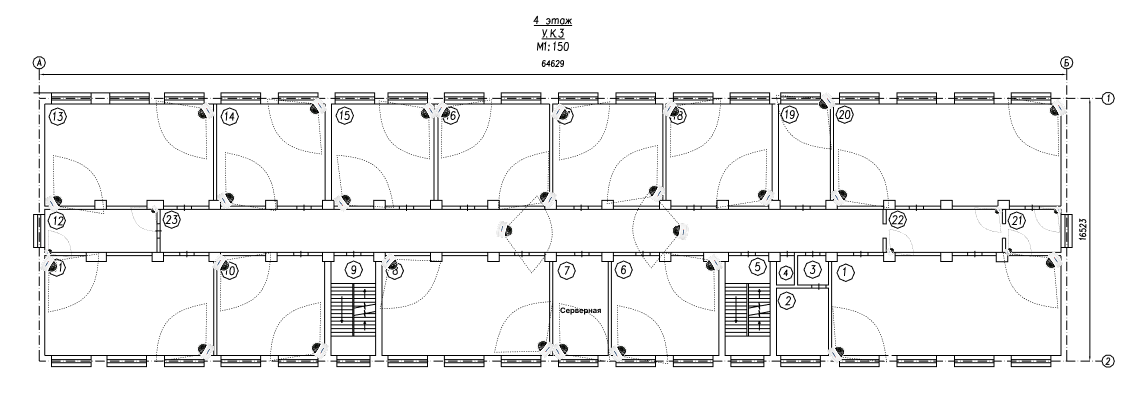
\includegraphics[width=240mm]{images/План размещения видеокамер}
    \end{center}
    \captionsetup{justification=centering}
    \caption{План размещения видеокамер}
    \label{fig::videocameras_placement}
\end{sidewaysfigure}


\subsection{Разработка схемы подключения оборудования}

Общее число используемых видеокамер составляет 34 штуки. К 1 коммутатору подключено 17 видеокамер, используется 2 коммутатора 
для подключения к видеокамерам и 1 коммутатор для объединения потока информации и передачи на основной сервер.

\begin{figure}[h]
    \begin{center}
        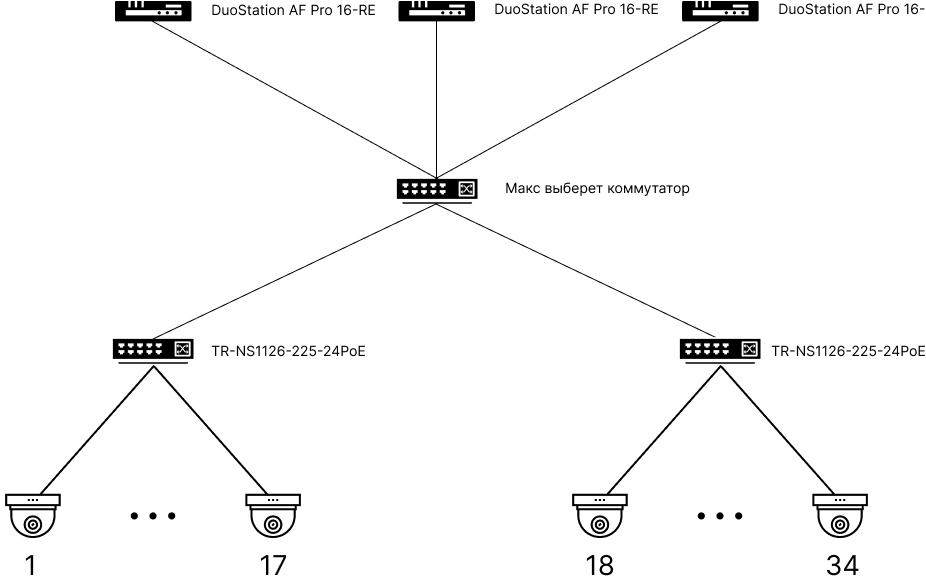
\includegraphics[width=160mm]{images/Схема подключения оборудования}
    \end{center}
    \captionsetup{justification=centering}
    \caption{Схема подключения оборудования}
    \label{fig::connections}
\end{figure}
